\chapter{Le moment angulaire orbital dans la génération d'harmoniques d'ordre élevé}
\label{CH:OAM_HHG}
%
\section{Génération d'harmoniques d'ordre élevé à partir de modes de Laguerre-Gauss}

Ayant passé en revue les utilisations envisagées de faisceaux de Laguerre-Gauss de durées ultra-brève et dans le domaine de l'extrême ultra-violet (XUV), nous décrirons ici comment les générer de manière expérimentale. Nous commencerons par détailler notre dispositif de génération d'harmoniques d'ordre élevé dans le cas habituel d'un mode laser Gaussien, puis expliquerons comment passer au cas Laguerre-Gaussien avant de donner les résultats obtenus.

\subsection{Le cas Gaussien : Aspects expérimentaux de la génération d'harmoniques d'ordre élevé}
\label{Sec:HHG_G}
\subsubsection{Système laser}
Toutes les expériences présentées dans ce chapitre ont été réalisées sur le laser LUCA (Laser Ultra-Court Accordable) du LIDYL au CEA Saclay. Il délivre des impulsions ayant une enveloppe temporelle gaussienne de largeur à mi-hauteur $\tau = 50$ fs et une enveloppe spatiale gaussien de largeur à mi-hauteur $w_0 = 15$ mm à $\frac{1}{e^2}$. La longueur d'onde utilisée est 800 nm, et le taux de répétition est de 20 Hz. Ce système dispose d'une fibre utilisée pour filtrer spatialement le faisceau, ce qui garantit un profil très proche d'un mode gaussien pur \mycite{MahieuAPB2015}. Le prix à payer est une diminution de l'énergie par impulsion, qui atteint quand même environ 35 mJ après la fibre et le dernier étage de compression.

\subsubsection{Génération d'harmoniques d'ordre élevé}
Nous commençons par mettre en forme le faisceau laser : son diamètre est ajusté à l'aide d'un iris et son énergie est ajustée grâce à un atténuateur constitué d'une lame demi-onde et d'une paire de polariseur croisés. \`{A} la sortie de cet atténuateur, la polarisation du laser est verticale (S). Le faisceau est ensuite focalisé par une lentille dans un jet de gaz délivré par une vanne pulsée à la fréquence du laser par un système piezo-électrique (Attotech). L'utilisation d'une vanne pulsée permet de n'envoyer du gaz que lorsque le faisceau laser est présent, ce qui limite la pression résiduelle dans les chambres à vide. Ainsi, on peut atteindre une pression assez élevé (XXX) dans la région focale sans que l'émission harmonique ne soit réabsorbée par le gaz résiduel. Un autre paramètre important est le diamètre de l'orifice de la vanne (ici, 150 $\mu m$) : en choisissant un diamètre faible, on crée une extension supersonique du gaz ce qui garantit une longueur d'interaction faible avec le laser. On s'approche ainsi des conditions idéales d'un plan d'atomes, ce qui limite l'importance des effets d'accord de phase dans la GHOE. \par
Le choix du gaz dépend de l'expérience réalisée : on peut par exemple utiliser une molécule dont on étudie la réponse, on parle alors de spectroscopie harmonique. Le gaz n'est pas l'objet d'étude dans notre cas, on préférera donc choisir un système simple, facile à se procurer, et ayant une grande section efficace. Le gaz le plus courant est l'Argon, qui est peu coûteux et génère de manière très efficace. Son potentiel d'ionisation est de 15.76 eV, ce qui donne une énergie de coupure assez faible et qui empêche de générer des ordres harmoniques très élevés. Dans les cas où on désire générer des ordres élevés et nombreux, on pourra utiliser d'autres gaz rares comme le Néon ($I_p$ = 21.6 eV) même si la génération sera moins efficace.

Pour notre système, les paramètres nominaux sont :
\begin{itemize}
\item Le diamètre avant focalisation \O{} $\approx$ 10-15 mm,
\item L'énergie par impulsion de l'ordre de E = 1 mJ,
\item La lentille de longueur focale f = 1 m. \\
\end{itemize}
Pour calculer la valeur de l'intensité pic au foyer, on peut calculer le profil du faisceau après focalisation, par exemple par un calcul numérique. Le champ avant la lentille est défini dans les coordonnées cylindriques $(R,\theta)$ par :
\begin{equation*}
E(R,\theta) = \sqrt{I_0} \exp{\left(-\frac{R^2}{w_0^2}\right)}\times\delta(\frac{\mbox{\O}}{2}-R),
\end{equation*}
où $w_0$ est la largeur du faisceau collimaté avant l'iris, \O{}  est le diamètre de l'iris, $\delta$ est la fonction de Heaviside, et $I_0 = \frac{2E\sqrt{\frac{4\log{2}}{\pi}}}{\tau\pi w_0^2}$.
La focalisation d'un faisceau par une lentille mince peut être calculée par une transformée de Fourier (voir \mycite{Goodman}, un des ouvrages de référence pour l'optique de Fourier, et \mycite{Tan} pour des exemples d'implémentations numériques). Il est alors simple de voir l'effet des différents paramètres expérimentaux. Par exemple, on peut faire varier le diamètre de l'iris : la Figure \ref{Fig:IrisScan} montre le profil du faisceau au foyer quand \O{} varie entre 5 et 25 mm. On voit alors que l'intensité pic au foyer évolue entre 0 et 10 $\times 10^{14} \mbox{W/cm}^2$. On se trouve donc parfaitement dans le régime d'intensité nécessaire à la génération d'harmonique : l'intensité est suffisante pour enclencher une ionisation tunnel mais reste assez faible pour ne pas ioniser et dépléter tout le milieu.

\begin{figure}[!ht]
\centering
\def\svgwidth{\columnwidth}
\import{Figures/Iris_Scan/}{Fig_IrisScan.pdf_tex}
\caption{\'{E}volution du foyer lorsqu'on varie la taille de l'iris. De gauche à droite : (1) profil transverse de l'intensité au foyer, (2) intensité pic, (3) taille du waist. Les paramètres sont les suivants : E = 1 mJ, $w_0$ = 15 mm, $\tau$ = 50 fs, $\lambda$ = 792 nm, f = 1 m et \O{} variant de 5 à 25 mm par pas de 1 mm. Le calcul est réalisé sur une grille de 1025x1025 points correspondant à une taille réelle de 5*\O{}.}
\label{Fig:IrisScan}
\end{figure}

Les harmoniques d'ordre élevé du laser infrarouge sont ainsi générées par le gaz situé près du foyer de la lentille. Ce rayonnement XUV est ensuite ré-imagé par un dispositif composé de deux optiques :
\begin{enumerate}
\item Un miroir torique en or de 50 cm de focale. Le miroir travaille à $11.5\degres$ d'incidence rasante ($78.5\degres$ si on défini l'angle par rapport à la normale au miroir), ce qui permet d'avoir une réflectivité importante et plate sur la gamme spectrale considérée (voir Figure \ref{Fig:TorR}).

\begin{figure}[!ht]
\centering
\def\svgwidth{0.6\columnwidth}
\import{Figures/Reflect_Torique/}{torR.pdf_tex}
\caption{Réflectivité calculée du miroir torique en or à un angle d'incidence de $11.5\degres$. (CXRO, \mycite{Henke1993}).}
\label{Fig:TorR}
\end{figure}

Le miroir toroïdal est positionné dans une configuration 2f-2f de sorte à garder un rapport 1:1 entre le foyer de génération et le second foyer. Ré-imager le foyer de génération est utile car on peut focaliser le rayonnement harmonique dans un deuxième dispositif, comme par exemple un spectromètre à temps de vol dans le cas d'une mesure RABBIT (voir ChapitreXX et YY). Un autre avantage est qu'il éloigne la zone de génération, où la pression est élevée, de la zone de détection, qui requiert souvent un vide de qualité pour que les détecteurs fonctionnent.\\

\item La deuxième optique est une lame de Si$\mbox{O}_{\mbox{2}}$, qui réalise le rôle de filtrage de l'infrarouge de génération. La lame de silice est traitée antireflet pour l'infrarouge grâce à un dépôt de multicouches. La dernière de ces couches est en silice, ce qui combiné à une bonne qualité de surface permet de réfléchir efficacement le rayonnement harmonique. La Figure \ref{Fig:SilR}, tirée de \mycite{MairessePhD} présente la réflectivité de la lame pour le rayonnement harmonique et infrarouge. La réflectivité dans l'XUV est donc supérieure à 50\% jusqu'à l'ordre $\approx 37$, tandis que moins de 10\% de l'infrarouge est réfléchi. Le filtrage de l'infrarouge de génération est souvent crucial : il constitue un bruit de mesure non négligeable, sans compter qu'il peut facilement endommager des optiques ou des détecteurs en aval s'il est focalisé.

\begin{figure}[!ht]
\centering
\def\svgwidth{\columnwidth}
\import{Figures/Reflect_Silice/}{silR.pdf_tex}
\caption{Réflectivité de la lame de silice. \`{A} gauche, transmission et réflectivité à 800 nm en fonction de l'angle d'incidence rasante. Les pointillés repèrent notre angle de $11.5\degres$. \`{A} droite, réflectivité XUV mesurée (cercles) et donnée par le CXRO (lignes) (\mycite{Henke1993}). Figure adaptée de \mycite{MairessePhD}.}
\label{Fig:SilR}
\end{figure}
\end{enumerate}

Nous souhaiterions ensuite pouvoir imager le spectre harmonique, c'est-à-dire séparer les différents ordres harmoniques et mesurer leurs propriétés spatiales. Un peu après le second foyer, les harmoniques sont dispersées par un réseau à pas variable Hitachi 001-0437 (voir \mycite{KitaAO1983} pour des détails sur son fonctionnement). L'angle de réflexion d'un rayonnement monochromatique de longueur d'onde $\lambda$ est donné par la formule des réseau :
\begin{equation*}
m\lambda=\frac{\sin{\alpha}+\sin{\beta}}{\sigma},
\end{equation*}
où $m$ est l'ordre de diffraction considéré (généralement 1), $\sigma$ le nombre de trait par mètre (1200 traits/mm dans notre cas), $\alpha$ et $\beta$ les angles d'incidence et de réflexion, définis par rapport à la normale au réseau (la documentation donne $\alpha = 87$\degres{} pour un fonctionnement optimal).\par
Le réseau de diffraction est cylindrique : il est focalisant dans la dimension horizontale mais est plan dans la direction verticale. Un rayonnement gaussien de faible largeur spectrale $\Delta\lambda$ et de largeur spatiale $w(z)$ formera donc dans le plan focal du réseau une fine ligne verticale de largeur proportionnelle à $\Delta\lambda$ et de hauteur $w(z)$. On image ainsi à la fois les dimensions spectrale et spatiale, si on suppose la symétrie cylindrique. Ce spectre est imagé par des galettes de micro-canaux couplées à un écran de phosphore, lui-même observé par une caméra CCD Basler A102f. 

L'intégralité du dispositif expérimental est représenté sur la Figure \ref{Fig:ExpG}.
\newpage
\vspace{\baselineskip}
\begin{figure}[!ht]
\centering
\def\svgwidth{\columnwidth}
\import{Figures/Setup_G/}{setupG_wbitmap.pdf_tex}
\caption{Dispositif expérimental de génération et détection d'harmoniques d'ordre élevé.}
\label{Fig:ExpG}
\end{figure}

Les figures \ref{Fig:SpectrumGAr} et \ref{Fig:SpectrumGNe} présentent des spectres obtenus avec ce dispositif en utilisant respectivement l'argon et le néon comme gaz de génération. On observe les ordres harmoniques allant de 13 à 29 dans l'argon, et de 13 à 57 dans le néon, la différence d'énergie de coupure étant attendue puisque le néon a un $I_p$ plus élevé. Sur le spectre de l'argon, on observe clairement les deux trajectoires quantiques de la GHOE : une contribution sur l'axe correspond à la trajectoire courte et une plus divergente et moins intense correspond à la trajectoire longue. Dans le cas du néon, les conditions d'accord de phase utilisées favorisent la trajectoire courte. On remarque également que la divergence de la trajectoire courte (resp. longue) augmente (rep. diminue) avec l'ordre harmonique, jusqu'à ce que les deux trajectoires se confondent dans la coupure. Notons finalement la présence sur le spectre du néon de pics satellites autour des harmoniques les plus basses : il s'agit des harmoniques plus élevées diffractées au second ordre par le réseau.
\begin{figure}[!ht]
\centering
\def\svgwidth{\columnwidth}
\import{Figures/Spectrum_G/}{Spectrum_G_Ar.pdf_tex}
\caption{Spectre d'harmoniques d'ordre élevé générées dans l'argon à partir d'un mode laser gaussien.}
\label{Fig:SpectrumGAr}
\end{figure}
\begin{figure}[!ht]
\centering
\def\svgwidth{\columnwidth}
\import{Figures/Spectrum_G/}{Spectrum_G_Ne.pdf_tex}
\caption{Spectre d'harmoniques d'ordre élevé générées dans le néon à partir d'un mode laser gaussien.}
\label{Fig:SpectrumGNe}
\end{figure}

\subsection{Génération de modes de Laguerre-Gauss dans le visible et proche infrarouge}
Ayant décrit la génération ``habituelle'' d'harmoniques d'ordre élevé, décrivons maintenant l'expérience où le laser générateur possède un mode de Laguerre-Gauss, dont l'expression a été donnée au chapitre précédent (équation \ref{eq:lgmodes}). Les modes de Laguerre-Gauss possèdent un moment angulaire orbital bien défini grâce à leur phase hélicoïdale. Plus précisément, c'est le terme $e^{\rmi\ell\theta}$, également présent dans les modes de Bessel, qui leur confère cette propriété. Il sera question de l'index radial $p$ des modes de Laguerre-Gauss plus loin dans cette thèse, mais il n'a pour l'instant pas d'importance pour notre problème. La première question est donc de savoir comment produire un mode de Laguerre-Gauss d'index $(\ell_{IR},0)$ dans l'infrarouge. 

\subsubsection{Superposition de modes de Hermite-Gauss}
\label{sec:hg_modes}
Les faisceaux de LG étant des modes du champ électromagnétique, on peut d'abord penser à modifier le laser lui-même pour qu'il lase directement dans le mode désiré. En introduisant des éléments absorbants dans la cavité, il est a priori possible d'interdire la génération d'un mode Gaussien. En pratique, il est assez compliqué de sélectionner un mode de LG. Il est par contre assez simple de sélectionner un des modes de \textit{Hermite-Gauss}, qui sont les solutions de l'équation d'onde en coordonnées cartésiennes. Ces modes sont souvent appelés modes $\mbox{TEM}_{nm}$, pour ``Transverse Electro-Magnetic'', dont le mode Gaussien $\mbox{TEM}_{00}$ n'est simplement que le mode d'index le plus bas. Quelques uns de ces modes sont représentés sur la figure \ref{Fig:hgmodes}. En insérant simplement un fil vertical (resp. horizontal) dans la cavité laser, on bloque la génération du $\mbox{TEM}_{00}$ et on obtient un mode $\mbox{TEM}_{01}$ (resp. $\mbox{TEM}_{10}$).

\begin{figure}[!ht]
\centering
\def\svgwidth{\columnwidth}
\import{Figures/Mode_Converter/}{HG_Modes.pdf_tex}
\caption{Modes de Hermite-Gauss pour différentes valeurs de $(n,m)$. De gauche à droite, $(n,m) =$ (0,0), (1,0), (0,1), (2,0), (2,1), (3,3). Le code couleur est le même que celui de la figure \ref{Fig:LGModes} : la couleur donne la phase et la luminosité l'intensité.}
\label{Fig:hgmodes}
\end{figure}

Les faisceaux de Hermite-Gauss constituent également une base des modes du champ, dans laquelle on peut donc écrire les modes de Laguerre-Gauss. On peut montrer (\mycite{BeijersbergenOC1993}) que les composantes du mode $\mathcal{LG}_{\ell,p}$ sont égales aux composantes d'un mode $\mbox{TEM}_{nm}$ incliné à 45\degres{} avec $p = \mathrm{min}(m,n)$ et $\ell=m-n$, la seule différence étant l'ajout d'une phase de $\pi/2$ entre les différentes composantes successives. Par exemple pour $\ell = 1$,
\begin{align*}
\mbox{TEM}_{n,m}^{45\mbox{\degres}}&=\frac{1}{\sqrt{2}}\mbox{TEM}_{01}+\frac{1}{\sqrt{2}}\mbox{TEM}_{10} \mbox{ et}\\
\mathcal{LG}_{1,0}&=\frac{1}{\sqrt{2}}\mbox{TEM}_{01}+\frac{\rmi}{\sqrt{2}}\mbox{TEM}_{10}.
\end{align*}
Pour $\ell = 2$, 
\begin{equation*}
\mathcal{LG}_{2,0}=\frac{1}{2}\mbox{TEM}_{02}+\frac{\rmi}{\sqrt{2}}\mbox{TEM}_{11}-\frac{1}{\sqrt{2}}\mbox{TEM}_{20}
\end{equation*}
et ainsi de suite.
Comme dit plus haut, il est possible de générer un mode $\mbox{TEM}_{n,m}$ en cavité, il reste seulement à l'incliner à 45\degres par rapport au repère choisi. Pour contrôler la phase entre les composantes relatives, les auteurs de \mycite{BeijersbergenOC1993} ont montré qu'on pouvait utiliser des lentilles cylindriques. En effet, une lentille cylindrique convergente ne focalise qu'une seule des composantes cartésiennes, qui va subir un déphasage au passage du foyer dû à la phase de Gouy. On recollimate ensuite le faisceau avec une deuxième lentille cylindrique de même focale $f$. La phase ajoutée est ajustée en changeant la distance entre ces deux lentilles; pour obtenir $\pi/2$ il faut choisir $\sqrt{2}f$. La Figure \ref{Fig:Modeconv} illustre le principe de ce dispositif, appelé convertisseur de mode.

\begin{figure}[!ht]
\centering
\def\svgwidth{0.5\columnwidth}
\import{Figures/Mode_Converter/}{mode_converter.pdf_tex}
\caption{Schéma de fonctionnement d'un convertisseur de mode : en partant d'un $\mbox{TEM}_{01}$ incliné à 45\degres, on obtient un mode $\mathcal{LG}_{1,0}$. Tiré de \mycite{PadgettAllen1999}.}
\label{Fig:Modeconv}
\end{figure}

L'intérêt de ce dispositif est de créer des modes purs : on obtient exactement le faisceau de Laguerre-Gauss recherché. Il présente cependant deux inconvénients : (1) il faut disposer d'un mode $\mbox{TEM}_{0\ell}$ au départ, ce qui devient compliqué dès que $\ell$ augmente. De plus, il est peu pratique de devoir modifier la cavité laser, particulièrement dans le cas des lasers de puissances utilisés pour la HHG. (2) Le faisceau est focalisé dans une dimension entre les deux lentilles. La puissance fournie par notre laser imposerait de réaliser la conversion dans une enceinte à vide, sans quoi la focalisation dans l'air détruira le profil spatial et temporel du faisceau. Pour ces raisons, nous avons choisi une méthode plus flexible et plus adapté à un laser de puissance.

\subsubsection{Utilisation d'une lame de phase à spirale}
Cette technique est probablement la façon la plus intuitive d'ajouter le terme de phase qui nous intéresse au faisceau. Pour rajouter une phase $e^{\rmi\ell\theta}$, il suffit d'utiliser une lame de verre transparente dont l'épaisseur varie proportionnellement à $\theta$. On forme ainsi une \textit{lame de phase à spirale} (Spiral Phase Plate, SPP), concept proposé dans \mycite{BeijersbergenOC1994} et représenté sur la Figure \ref{Fig:SPP}.\par
\begin{figure}[!ht]
\centering
\def\svgwidth{0.5\columnwidth}
\import{Figures/SPP/}{SPP.pdf_tex}
\caption{Lame de phase à spirale. La flèche rouge représente le trajet d'un rayon optique. Adapté de \mycite{YaoAOP2011}.}
\label{Fig:SPP}
\end{figure}
La lame présente une discontinuité pour $\theta=0$\degres, dont la hauteur h permet de contrôler le moment angulaire orbital transféré au faisceau pour une longueur d'onde donnée. Si cette hauteur est assez faible pour que l'on reste dans le régime paraxial, on peut considérer que la lame agit uniquement sur la phase du faisceau incident. Ainsi si on choisit 
\begin{equation*}
h = \frac{\ell\lambda}{n-1},
\end{equation*}
où $n$ est l'indice de réfraction du milieu, pour un champ d'entrée $u(r,\theta,z)$ on obtient directement après la lame $u' = u\exp{(-\rmi \ell \theta)}$.	Il est donc non seulement possible de passer d'un mode Gaussien à un mode Laguerre-Gaussien, mais encore de changer l'indice d'un mode déjà Laguerre-Gaussien.\par
La lame de phase illustre joliment la création de MAO : si on considère une onde plane arrivant perpendiculairement à la surface plane de la lame, le rayon qui sort de la lame sera dévié par réfraction à travers la surface hélicoïdale. Cette réfraction se fait dans la direction azimutale, le moment linéaire de la lumière acquière donc une composante azimutale, synonyme de moment angulaire. Plus précisément, pour un rayon $r$ donné, l'angle de la surface	vaut $h/(2\pi r)$. Si on applique la loi de Snell-Descartes on obtient que le rayon est dévié d'un angle $\alpha = (n-1)\ell\lambda/(2\pi r(n-1)) = \ell/(k_0r)$. Le moment linéaire par photon vaut $\hbar k_0$, donc le moment angulaire par photon vaut $r\times\hbar k_0\times\ell/(k_0r) = \ell\hbar$.


Si le principe d'une SPP est simple, sa construction est beaucoup plus compliquée. Les tolérances sur la valeur de h et la régularité de la surface sont très strictes aux longueurs d'ondes optiques, sans quoi la qualité du mode de sortie sera détériorée (si h n'est pas adapté, on peut même créer des modes d'indice non entier, cf. \mycite{LeachNJP2004}). D'ailleurs, lors des premiers travaux sur le sujet (\mycite{BeijersbergenOC1994}), la température de la lame était ajustée pour accorder précisément la hauteur de la lame à la longueur d'onde. La technique a évolué et il est maintenant possible de créer des SPP de très bonne qualité \mycite{OemrawsinghAO2004}.

Enfin, remarquons que même pour une SPP parfaite, la conversion d'un mode à l'autre n'est jamais idéale. La SPP agit sur la phase du faisceau, mais ne modifie pas le profil d'intensité. Ainsi, à sa sortie le champ électrique a la bonne phase mais pas la distribution d'intensité d'un mode de Laguerre-Gauss (termes sur la première ligne de l'équation \ref{eq:lgmodes}). La conséquence est que le champ $u_{exp}$ créé n'est pas un mode pur du champ, mais une superposition de modes de Laguerre-Gauss de différents indices. Ainsi, son intensité sera fortement modulée au cours de la propagation selon la phase entre ces différents modes. Le cas qui nous intéresse principalement est la conversion d'un mode Gaussien vers un mode LG. Dans ce cas, cette superposition s'écrit :
\begin{align}
\begin{split}
u_{exp}(r,\theta,z) &= \sum_{p=0}^\infty\sum_{\ell=-\infty}^\infty{\Braket{u_{exp}(r,\theta,z)|\mathcal{LG}_{\ell,p}(r,\theta,z)} \ket{\mathcal{LG}_{\ell,p}(r,\theta,z)}}\\
&=\sum_{p=0}^\infty\sum_{\ell=-\infty}^\infty{\Braket{TEM_{00}(r,\theta,z)\cdot e^{\rmi\ell'\theta}|\mathcal{LG}_{\ell,p}(r,\theta,z)} \ket{\mathcal{LG}_{\ell,p}(r,\theta,z)}},
\end{split}
\label{Eq:decompLG}
\end{align}
où $\ell'$ est l'indice azimutal correspond à la hauteur de la SPP. Les coefficients sont simplement donnés par le produit scalaire ci-dessus. On remarque qu'il a la forme suivante :
\begin{equation*}
\Braket{TEM_{00}(r,\theta,z)\cdot e^{\rmi\ell'\theta}|\mathcal{LG}_{\ell,p}(r,\theta,z)} = \int_{r=0}^\infty\int_{\theta=0}^{2\pi}{\ldots \; e^{\rmi(\ell'-\ell)\theta}r\rmd r \rmd \theta},
\end{equation*}
l'intégrale selon $\theta$ s'annule donc dès que $\ell\neq\ell'$. Les modes de la superposition ont donc tous le même index azimutal mais des $p$ différents. Ces coefficients peuvent être calculés numériquement, par exemple \mycite{BeijersbergenOC1994} obtiennent pour le cas $\ell' = 1$ les valeurs présentées dans le Tableau \ref{Tab:DecompBei}. On conclut donc que le faisceau est composé majoritairement du mode $\mathcal{LG}_{1,0}$. Les valeurs deviennent moins bonne lorsqu'on augmente $\ell$, par exemple un Gaussien passant à travers une lame dessinée pour ajouter $\Delta\ell =2$ n'est composé qu'à 50\% du mode $\mathcal{LG}_{2,0}$ recherché.
\begin{center}
  \begin{tabular}{ c | c | c | c | c | c | c }
    \hline
		& $p = 0$ & 1 & 2 & 3 & 4 & 5 \\ \hline
    $\ell=1$ & 78.5 & 9.82 & 3.68 & 1.92 & 1.17 & 0.79 \\ \hline
  \end{tabular}
	\caption{Décomposition du champ obtenu en passant un mode Gaussien pur à travers une lame de phase à spirale. D'après \mycite{BeijersbergenOC1994}.}
	\label{Tab:DecompBei}
\end{center}
Pour finir, mentionnons une technique permettant de relâcher un peu les contraintes de fabrication d'une SPP : il est possible de discrétiser la pente de phase, ce qui rend la lame plus facile à construire et donc plus accessible. Cette technique est détaillée dans \mycite{SuedaOE2004}, où les auteurs calculent l'influence du nombre de points de discrétisation sur la pureté modale obtenue :
\begin{center}
  \begin{tabular}{c | c | c | c | c | c}
    \hline
		Nombre de points de discrétisation & $\infty$ & 32 & 16 & 8 & 4 \\ \hline
    Efficacité $\mathcal{LG}_{0,0}\rightarrow\mathcal{LG}_{1,0}$ & 78.5 & 78.3 & 77.5 & 74.6 & 63.7 \\ \hline
  \end{tabular}
	\caption{Efficacité de conversion d'une lame de phase à spirale $\Delta\ell=1$ en fonction du niveau de discrétisation. D'après \mycite{SuedaOE2004}.}
	\label{Tab:DecompSueda}
\end{center}
La qualité du mode obtenue est donc très correcte même jusqu'à 8 niveaux. Les auteurs montrent également que ces lames de phase sont adaptées à des utilisations avec des faisceaux courts et intenses, contrairement à la plupart des autres méthodes. Pour ces raisons, nous avons finalement choisi d'utiliser une lame de phase discrétisée sur 16 niveaux, et disposons de lames $\Delta\ell = 1$ et $\Delta\ell = 2$ à 800 nm, ce qui nous permet d'aller jusqu’à $\ell = 3$ en les mettant l'une après l'autre.

\subsubsection{Résultats expérimentaux sur la création de modes de Laguerre-Gauss dans l'infrarouge}
Même si le système laser a été décrit plus haut, notons encore une fois l'importance du filtrage spatial installé sur notre chaîne : il nous garantit un mode Gaussien très pur, ce qui favorise grandement la création de modes Laguerre-Gaussien de qualité. \par
Les lames de phases utilisées ont été construites par la société Silios Technologies et font 17 mm de diamètre. Elle ou elles sont insérées directement après l'iris et avant la lentille. Le faisceau étant bien collimaté, nous n'avons pas observé de différence notable selon le placement de la lame. Il est intéressant d'observer l'intensité du faisceau un peu après le passage dans la lame : 

\begin{figure}[!ht]
\centering
\def\svgwidth{0.4\columnwidth}
\import{Figures/SPP/}{Beam_1m_After_SPP.pdf_tex}
\caption{Intensité transverse après être passée dans une lame de phase à spirale $\Delta\ell = 1$. Le faisceau est d'abord diaphragmé par un iris de diamètre 10 mm, la distance d'observation après la lame est de 1 m.}
\label{Fig:BeamAfterSPP}
\end{figure}

On observe 16 ``pétales'' sur les bords du faisceau, qui correspondent à la diffraction par les 16 marches de la lame. On voit également la singularité de phase déjà formée, qui donne un zéro d'intensité au centre. Clairement, l'intensité du faisceau est encore très loin de celle d'un mode de Laguerre-Gauss : il n'y a que dans le champ lointain que le faisceau prendra la forme désirée. Dans notre cas, cela se passe au foyer de la lentille de génération. Nous imageons ce foyer à l'aide d'une caméra CCD Imagine Source équippée d'un objectif x5 et d'un tube de 160 mm. La figure \ref{Fig:LGFocus} présente les résultats obtenus.\par
\begin{figure}[!ht]
\centering
\def\svgwidth{0.8\columnwidth}
\import{Figures/IRFocus/}{SPP1focus.pdf_tex}
\caption{Intensité laser au foyer d'une lentille de 1m, après passage à travers (1) une lame de phase $\Delta\ell = 1$, (2) une lame de phase $\Delta\ell = 2$, et (3) les deux lames placées successivement.}
\label{Fig:LGFocus}
\end{figure}
On mesure le diamètre de l'anneau, défini comme la distance entre les deux maxima d'intensité le long d'une ligne radiale, et on obtient 200, 280 et 400 \si{\um} pour $\ell=$1, 2, 3. Ceci est cohérent avec la dépendance en $\sqrt{\ell}$ attendue (voir équation \ref{Eq:rmax_LG}), mais ne constitue pas une mesure directe du MAO porté par le faisceau. Pour ce faire, il existe de nombreuses techniques développées dans le domaine visible et infrarouges dont le but est toujours de révéler le terme de phase $\mathrm{e}^{\rmi\ell\theta}$. Pour révéler cette phase spatiale, il est naturel d'essayer d'observer des interférences, soit avec un autre faisceau - l'interférence avec un gaussien donne une ``fourche'' d'ordre $\ell$ \mycite{bazhenov1990} - ou bien du faisceau avec lui même, c'est-à-dire sa diffraction. De nombreux objets diffractifs ont été utilisés, par exemple une fente \mycite{ghai2009} ou des fentes de Young \mycite{sztul2006}, avec lesquelles le signe et la parité de $\ell$ se retrouvent dans le décalage des franges, ou bien des objets plus compliqués tels que des grilles de pupilles \mycite{berkhout2008} qui donnent directement la valeur de $\ell$. On peut également mentionner les ouvertures bloquant une partie angulaire du faisceau, ce qui se répercute sur le contenu modal du faisceau à travers la relation d'incertitude $\Delta\ell\Delta\phi > K$ déjà mentionnée (TODO). Certaines méthodes sont généralisables au cas d'un photon unique et ont permis de mesurer de l'intrication entre différents états de moment orbital angulaire \mycite{MairNature2001} ainsi qu'un équivalent angulaire au paradoxe EPR \mycite{LeachScience2010}. \par 
Nous avons choisi d'utiliser une ouverture en triangle, qui donne une figure de diffraction assez surprenante : on obtient une grille de points diffractés en forme de triangle, dont l'orientation donne le  signe de $\ell$ alors que le nombre de points donne $\left|\ell\right|$ : sur l'arête extérieure au triangle, on a $\left|\ell\right|+1$ points \mycite{HickmannPRL2010}. Après être passé dans la SPP, le faisceau est diffracté par une ouverture triangulaire dont la taille est ajustable à l'aide d'un système motorisé conçu par M. Bougeard. On choisit l'ouverture de l'ordre du waist du faisceau, ce qui permet d'observer la figure de diffraction en imageant le foyer d'une lentille de focale f=1m. La figure \ref{Fig:Triangle} illustre le principe et les résultats de cette expérience. 

\begin{figure}[!ht]
\centering
\def\svgwidth{1.0\columnwidth}
\import{Figures/Triangle/}{triangle.pdf_tex}
\caption{Mesure directe du moment angulaire orbital porté par le faisceau infrarouge à l'aide d'une ouverture triangulaire.}
\label{Fig:Triangle}
\end{figure}

Nous avons pu vérifier la validité de cette méthode pour des moments angulaires plus élevés. Pour les obtenir, le champ infrarouge $E_{800}$ est doublé à l'aide d'un cristal de BBO (bêta-borate de baryum). On obtient un champ à 400 nm, dont l'amplitude est donné par la loi habituelle de l'optique non-linéaire perturbative $E_{400}\propto E_{800}^2\propto \rme^{2\rmi\ell_{IR}\theta}$. Le MAO du faisceau est ainsi doublé, comme vérifié expérimentalement par \mycite{DholakiaPRA1996}. Les résultats obtenus après diffraction par la fente triangulaire sont présentés sur la figure \ref{Fig:Triangle400}. 

\begin{figure}[!ht]
\centering
\def\svgwidth{0.5\columnwidth}
\import{Figures/Triangle/}{triangle400.pdf_tex}
\caption{Mesure directe du moment angulaire orbital porté par le champ obtenu après doublage du faisceau infrarouge dans un cristal de BBO.}
\label{Fig:Triangle400}
\end{figure}

Ceci constitue donc une preuve directe que le faisceau est composé très majoritairement du mode $\mathcal{LG}_{\ell,0}$. Bien sûr, on ne s'attend quand même pas à ce que les modes obtenus soient purs, du fait de la lame de phase mais également à cause de l'iris qui limite la dimension transverse du faisceau. On peut évaluer numériquement l'effet de tous ces éléments : on effectue un calcul de propagation de la même façon qu'expliqué en page \pageref{Fig:IrisScan}, cette fois en rajoutant l'effet de la lame de phase discrète. Une fois le foyer obtenu, on calcule sa décomposition dans la base des modes de Laguerre-Gauss en évaluant numériquement les coefficients du type \ref{Eq:decompLG}. Comme noté page \pageref{Eq:rmax_LG}, les modes de Laguerre-Gauss ne constituent une base que pour une valeur de $w(z)$ donnée. Il faut donc choisir cette valeur avant d'effectuer la décomposition. On fait l'hypothèse que le mode obtenu est assez proche d'un mode pur $(\ell,0)$ pour que son rayon soit donné par l'équation \ref{Eq:rmax_LG}, ce qui nous permet de fixer $w(z)$. La figure \ref{Fig:DecompIR} montre l'intensité au foyer et les coefficients de la décomposition ainsi obtenus. On voit que le foyer est composé du mode $\mathcal{LG}_{\ell,0}$ à 72, 48 et 42\% pour $\ell=1,2,3$ respectivement. On observe également l'apparition d'un deuxième anneau pour $\ell =2$ et 3, dû au vignetage du faisceau par l'iris et cohérent avec la présence de davantage de modes $p$. \par

\begin{figure}[!ht]
\centering
\def\svgwidth{\columnwidth}
\import{Figures/Mode_Decomposition_IR/}{mode_L123.pdf_tex}
\caption{Intensité laser au foyer d'une lentille de 1m, après passage à travers (1) une lame de phase $\Delta\ell = 1$, (2) une lame de phase $\Delta\ell = 2$, et (3) les deux lames placées successivement.}
\label{Fig:DecompIR}
\end{figure}

Nous concluons donc que même si le contenu modal devient moins pur à mesure que $\ell$ augmente, le mode dominant reste celui qui nous intéresse. La GHOE étant un processus très non-linéaire, c'est lui qui contribuera majoritairement. 

\subsection{Génération d'harmoniques d'ordre élevé d'un faisceau de Laguerre-Gauss}
\subsubsection{Contraintes expérimentales}
\label{sec:contraintes}
Une fois qu'on dispose d'un faisceau infrarouge de MAO défini, l'expérience ne diffère en principe pas du cas Gaussien présenté dans la partie \ref{Sec:HHG_G}. En pratique, un problème important subsiste : celui de l'intensité pic. Nous avons vu que pour générer des harmoniques d'ordre élevé, l'intensité au foyer doit être de l'ordre de $\SI{1e14}{W/cm^2}$. Pour un mode de Laguerre-Gauss d'index $(\ell,0)$, l'intensité maximale est obtenue en $r_\mathrm{max}$ (équation \ref{Eq:rmax_LG}) :
\begin{align*}
I_\ell(r_\mathrm{max},z=0) &= \frac{C_{\ell,0}^2}{{w_0}^2}{\left( {\frac{r_\mathrm{max}\sqrt{2}}{{w_0}}} \right)^{2\left| \ell  \right|}}{e^{\left( { - \frac{{2{{r_\mathrm{max}}^2}}}{{{{w_0}^2}}}} \right)}}\\
&= \frac{2}{\pi(1+\delta_{0\ell})\left| \ell  \right|!{w_0}^2}\ell^{\left| \ell  \right|}{e^{-\ell}}
\end{align*}
La formule de Stirling donne $\left| \ell  \right|!\approx\sqrt{2\pi\left| \ell  \right|}\left| \ell  \right|^{\left| \ell  \right|}e^{-\left| \ell  \right|}$. Elle est valable respectivement à 8\%, 4\% et 2.6\% près pour $\ell=1,\;2,\;3$. On peut donc approximer :
\begin{equation*}
I_\ell(r_\mathrm{max},z=0) \approx \frac{2}{\pi{w_0}^2}\frac{1}{\sqrt{2\pi\left| \ell  \right|}}\text{ pour }\ell\neq0. 
\end{equation*}  
L'intensité pic évolue donc en $1/\sqrt{\left| \ell  \right|}$, la génération est donc de plus en plus compliquée à mesure que le MAO de l'infrarouge $\ell_{1}$ augmente. Si on évalue l'expression exacte ci-dessus, on obtient :

\begin{center}
  \begin{tabular}{ c | c | c | c | c }
    \hline
		$\ell_{1}$ & 0 & 1 & 2 & 3 \\ \hline
    $I_{\mathrm{max}}$ & 1 & 0.7358 & 0.5413 & 0.4481 \\ \hline
  \end{tabular}
	\caption{Intensité pic d'un mode de Laguerre-Gauss en fonction de $\ell$. Les intensités sont normalisées à celle du mode $\ell = 0$.}
	\label{tab:ipeaklg}
\end{center}
Nous avons la chance de disposer d'un laser assez énergétique (jusqu'à 35 mJ disponibles), qui comme on le verra est suffisant pour générer jusqu'à $\ell_{1}=3$. Il est également probable que l'accord de phase s'effectue différemment avec un faisceau de LG, mais ces effets sont minimisés dans notre dispositif par l'utilisation d'un jet de gaz pulsé fournissant un milieu très fin.

La seconde contrainte expérimentale est due au système d'imagerie. Comme démontré plus haut, le faisceau infrarouge est constitué d'un mode de Laguerre-Gauss principal. Le principe de conservation du moment angulaire nous amène à penser que les harmoniques générées doivent également porter du MAO, et prendront donc problablement la forme de modes de Laguerre-Gauss. Nous avons vu dans la partie \ref{sec:hg_modes} que les modes de Laguerre-Gauss peuvent être vus comme la superposition de plusieurs modes d'Hermite-Gauss et que le déphasage entre ces modes était crucial. En particulier, le convertisseur de mode présenté sur la figure \ref{Fig:Modeconv} repose sur l'utilisation de lentilles cylindriques pour contrôler la phase d'un seul des modes de Hermite-Gauss. On comprend donc que n'importe quel élément optique focalisant différemment les deux composantes cartésiennes du champ va modifier la phase relatives des modes HG et détruire le mode de Laguerre-Gauss. Dans notre dispositif présenté sur la figure \ref{Fig:ExpG}, on trouve deux éléments problématiques :

\begin{itemize}
\item Les optiques de focalisation peuvent être astigmatiques. En particulier, la lentille de focalisation et le miroir torique doivent être alignés parfaitement, sans quoi notre mode en sera perturbé.\\
\item Le réseau de diffraction du spectromètre est un réseau cylindrique, il va donc systématiquement détruire le profil du faisceau au passage de son foyer.\\
\end{itemize}

L'effet du réseau de diffraction cylindrique peut être calculé. Par exemple, \mycite{VaityPLA2013} proposent d'utiliser l'astigmatisme introduit par une lentille inclinée pour mesurer le MAO porté par un faisceau. Nous adaptons ici leur formalisme au cas de notre réseau de diffraction. Considérons par simplicité un faisceau collimaté incident sur le réseau de diffraction. Pour décrire sa propagation, on peut utiliser les matrices de transfert. La matrice totale du système est
\begin{equation*}
M_{\mathrm{tot}} = M_{z_1}\cdot M_{\mathrm{r\acute{e}seau}}\cdot M_{z_0}\;,
\end{equation*}
où $z_0$ est la distance de propagation en amont du réseau, $z_1$ la distance en aval, $M_z$ et $M_{\mathrm{r\acute{e}seau}}$ décrivent respectivement la propagation sur une distance $z$ et la focalisation par le miroir :
\begin{equation*}
M_z = \left(
\begin{array}{cc}
	I & zI \\
	0 & I
\end{array} \right)\text{ avec } 
I = \left(
\begin{array}{cc}
	1 & 0 \\
	0 & 1
\end{array} \right)
\end{equation*}


\begin{equation*}
M_{\mathrm{r\acute{e}seau}} = \left(
\begin{array}{cc}
	I & 0 \\
	-C/f & I
\end{array} \right)\text{ avec } 
C = \left(
\begin{array}{cc}
	1 & 0 \\
	0 & 0
\end{array} \right).
\end{equation*}
$f$ est la longueur focale effective du réseau dans la direction horizontale. En fonction nominal, le réseau focalise horizontalement les harmoniques dans un plan appelé ''spectral'' situé 235 mm en aval \mycite{KitaAO1983}. Comme on considère ici un faisceau collimaté, on prendra $f$ = 235 mm.
\`{A} partir de $M_{\mathrm{tot}}$, l'équation (8) de \mycite{VaityPLA2013} donne l'expression analytique du champ à une distance $z_1$ du réseau :

\begin{equation}
E(x,y)=A(\rmi/2)^{|\ell|+1}\exp{\left[-(\beta_1 x^2+\beta_2 y^2)\right]}\times\gamma^{|\ell|} HG_\ell\left[(\alpha_1 x+\rmi\epsilon\alpha_2 y)/\gamma\right],
\label{eq:focusgrating}
\end{equation}
où $\ell$ est le MAO de l'harmonique considérée, $A$, $\beta_1$, $\beta_2$, $\alpha_1$, $\alpha_2$, $\gamma$ sont des constantes déterminées par les paramètres du problème, et $\epsilon=\pm1$ est le signe de $\ell$.

L'expression \ref{eq:focusgrating} contient un polynôme de Hermite d'ordre $\ell$, signe que le réseau agit comme un convertisseur de mode. Pour évaluer cette expression, choisissons par exemple l'harmonique 11 et supposons qu'elle porte un moment angulaire orbital bien défini. Considérons qu'elle soit collimaté et que son waist soit égal à 10 mm. La figure \ref{Fig:gratingfocus} représente l'intensité obtenue pour $z_1$ variant autour de 235 mm, en supposant $\ell_{11} = 3$ ou 11. Nous voyons d'abord qu'à l'écart du foyer, l'anneau est simplement focalisé dans la dimension spectrale (noter les échelles différentes en $x$ et $y$). Au foyer le faisceau prend la forme d'un mode de Hermite-Gauss d'index $\ell_{11}$ tourné à 45$\deg$ par rapport à l'axe du réseau. On ne peut donc pas imager le spectre harmonique en ce point comme dans le cas Gaussien. Cependant, si on s'écarte trop du plan spectral du réseau, les harmoniques ne sont plus séparées spatialement. De plus, leur intensité est moindre, ce qui rend la mesure plus difficile. Le compromis finalement choisi est de placer le détecteur 8 cm en amont du plan focal, ce qui donne des harmoniques séparées et un effet cylindrique peu visible (voir la section suivante).

\begin{figure}[!ht]
\centering
\def\svgwidth{1.1\columnwidth}
\import{Figures/Gratingfocus/}{gratingfocus.pdf_tex}
\caption{Intensité de l'harmonique 11 au voisinage du foyer du réseau de diffraction cylindrique, en supposant $\ell_{11} = 3$ (ligne du haut) et $\ell_{11} = 11$ (ligne du bas). La position longitudinale $z$ est indiquée au dessus des images. La dimension verticale est celle non focalisée par le réseau, et est donc plusieurs ordres de grandeurs plus large que la dimension horizontale. Notons également que l'échelle horizontale change d'une image à l'autre, de sorte à garder une image résolue.}
\label{Fig:gratingfocus}
\end{figure}

La dernière contrainte expérimentale est celle de la divergence du faisceau, qui évolue comme $\sqrt{\ell}$. Nous choisissons de réduire cette divergence en utilisant une lentille de focale f = 2 m, de sorte à ce que même si $\ell$ devient grand, les harmoniques ne soient pas tronquées par les optiques du dispositif. Le prix à payer étant bien sûr une intensité disponible au foyer plus faible. 

\subsubsection{Résultats}
\label{sec:results_lg}
Nous présentons sur la figure \ref{Fig:LGSpectrumAr} les spectres obtenus après les modifications expliquées ci-dessus effectuées, en utilisant $\ell_{1} = 1,\;2,\;3$. 

\begin{figure}[!ht]
\centering
\def\svgwidth{1\columnwidth}
\import{Figures/LGSpectrumAr/}{LGspectrum_ar.pdf_tex}
\caption{Intensité normalisée des harmoniques 13 à 25 générées dans l'argon et observées en champ lointain, en utilisant $\ell_{1} = 1$ (ligne du haut), $\ell_{1} = 2$ (ligne du milieu) et $\ell_{1} = 3$ (ligne du bas). Le détecteur (MCP) est placé 8 cm avant le plan spectral du réseau de diffraction, comme expliqué plus haut. Sur la droite, coupe de l'intensité le long de la ligne pointillée verticale blanche. Les lignes pointillées horizontales blanches représente la position moyenne des maxima des anneaux.}
\label{Fig:LGSpectrumAr}
\end{figure}

Nous observons donc une série d'harmoniques constituées d'un anneau. La première observation est que l'énergie de coupure diminue avec le MAO du laser de génération $\ell_{1}$, ce qui s'explique par la diminution de l'intensité pic (voir section \ref{sec:contraintes}). On rappelle que l'énergie de coupure est donnée par $I_c = I_p+3.17U_p$. $I_c$ pour $\ell_{1} = 1$ vaut environ $27*1.55=\SI{41.85}{eV}$. Si on utilise cette valeur et les rapports d'intensité pic données par le tableau \ref{tab:ipeaklg}, on obtient $I_c=\SI{34.91}{eV}$ et $I_c=\SI{31.59}{eV}$ pour $\ell_{1} = 2$ et 3. Ces valeurs sont comparables à celles de la figure \ref{Fig:LGSpectrumAr}, malgré la difficulté d'estimer précisément une énergie de coupure à partir d'un spectre d'harmoniques. 

Intéressons nous ensuite à la forme des harmoniques. Les anneaux sont elliptiques, effet du réseau de diffraction qui commence à focaliser dans la dimension horizontale. Une autre conséquence de la focalisation est que ne nous retrouvons pas strictement un zéro au centre des anneaux. On n'observe pas de sur-intensités selon la diagonale, signe que l'effet aberrant du réseau décrit plus haut est bien minimisé et que les optiques de transport sont correctement alignées.
On observe que le profil des anneaux se dégrade à mesure que $\ell_{1}$ augmente. La cause principale de cet effet est la conversion du mode $TEM_{00}$ en mode $\mathcal{LG}_{\ell_{1},0}$, qui comme vu plus haut devient mauvaise pour des $\ell_1$ élevés (voir la figure \ref{Fig:DecompIR}). Il est également possible que l'intensité plus faible au foyer des modes d'indices élevés nous force à utiliser un faisceau de diamètre avant focalisation plus grand et donc plus aberré.

Finalement, on remarque que l'émission harmonique n'est constituée que d'un seul anneau. Comme nous le verrons par la suite, cela signifie que seule la trajectoire quantique courte a un accord de phase favorable dans nos conditions expérimentales. On montrera également que dans ces conditions, le champ de chaque harmonique est constitué principalement d'un unique mode de Laguerre-Gauss. Enfin, remarquons que la divergence des harmoniques (dimension verticale) semble constante avec l'ordre harmonique, et ce pour chaque valeur de $\ell_{1}$. On mesure le diamètre moyen des anneaux, qui vaut $1.01\pm 0.02$ mm, $1.33\pm 0.04$ mm et $1.61\pm 0.01$ mm. 

Nous avons également pu effectuer cette expérience dans le Néon, le spectre obtenu avec $\ell_1=1$ est présenté sur la figure \ref{Fig:LGSpectrumNe}. Grâce à son potentiel d'ionisation plus élevé que l'Argon, on observe un spectre allant jusqu'à l'harmonique 41. Cependant, la génération est beaucoup moins efficace et nous n'avons pas réussi à atteindre l'intensité nécessaire lorsque le laser de génération portait $\ell_1=2,\;3$. Toutes les observations faites dans l'Argon sont valables : on observe bien des anneaux simples de diamètre constant, égal à $1.00\pm 0.05$ mm en moyenne.

\begin{figure}[!ht]
\centering
\def\svgwidth{1\columnwidth}
\import{Figures/LGSpectrumNe/}{LGspectrum_ne.pdf_tex}
\caption{Intensité normalisée des harmoniques 23 à 41 générées dans le néon et observées en champ lointain, en utilisant $\ell_{1} = 1$.}
\label{Fig:LGSpectrumNe}
\end{figure}

Les propriétés observées sont donc robustes : elles sont vérifiées pour plusieurs valeurs du MAO de l'infrarouge et dans des gaz différents. Nous allons voir dans la partie suivante qu'elles sont suffisantes pour démontrer la conservation du moment angulaire dans le processus de génération d'harmoniques.

\section{Conservation du moment angulaire orbital dans la GHOE}
\subsection{Vers une mesure non-interférométrique du moment angulaire orbital}
Comme vu dans le chapitre II, le moment angulaire est une quantité conservée. Dans l'interaction laser-matière que nous étudions, le MAO porté par le faisceau infrarouge doit être transféré soit à la matière, soit au faisceau harmonique généré. Il est donc crucial de parvenir à mesurer le MAO porté par chaque ordre harmonique du spectre. Deux équipes se sont déjà intéressées à ce problème :

\begin{itemize} 
\item \mycite{ZurchNP2012} ont été les premiers à utiliser des faisceaux de LG dans la GHOE. Ils ont pu étudier l'harmonique 11, et ont mesuré son MAO en la faisant diffracter sur un fil de tungsten de $\SI{5}{\micro\m}$. Le résultat de cette expérience est $\ell_{11}=1$.\\
\item \mycite{GariepyPRL2014} ont quant à eux choisi de créer deux sources d'harmoniques côte à côte, l'une Gaussienne, et l'autre Laguerre-Gaussienne. Ces deux sources génèrent chacune un spectre, et dans les bonnes conditions interfèrent spatialement. Dans les franges observées pour chaque harmonique, on voit une discontinuité dont l'ordre donne la différence de MAO entre les harmoniques générées par les deux sources. La source Gaussienne sert de référence, ce qui leur a permis de mesurer $\ell_{11}=11$, $\ell_{13}=13$, et $\ell_{15}=15$.\\
\end{itemize}

Les deux expériences sont clairement contradictoires. Elles ont toutes deux été effectuées dans des conditions de focalisation usuelles, où l'approximation paraxiale est valable. On s'attend donc à ce que les termes non-dipolaires soient totalement négligeables (voir section \ref{sec:selectionrules}), et que le processus de GHOE ne soit pas modifié à l'échelle microscopique. On aura alors la phase usuelle des harmoniques en fonction de celle de l'infrarouge : $\phi_q(r,\theta) = q\times\phi_1(r,\theta) = q\ell_1\theta$. Des simulations numériques plus précises \mycite{HernandezPRL2013} montrent également qu'en restant dans le cadre de la SFA, on obtient bien $\ell_{q}=q\times\ell_1$, ce qui est le résultat de Gariepy \textit{et al}. Cette loi de transfert reflète la conservation du MAO : il faut $q$ photons infrarouges pour générer un photon de l'harmonique $q$, qui doit donc porter $q\times\ell_1$ unités de MAO.
Toutefois, le résultat de Zürch \textit{et al.} a été obtenu dans des conditions de génération assez inhabituelles, avec un milieu long et une intensité élevée. Les auteurs expliquent l'écart aux prédictions théoriques en disant qu'initialement, les harmoniques portent bien un MAO de $q\times\ell_1$ mais qu'il est détruit par des effets de propagation, qui amènent à $\ell_q = 1$.

Si les conditions de génération sont si importantes dans la GHOE à partir de faisceaux de Laguerre-Gauss, il faut disposer de méthodes de caractérisation robustes. Les techniques utilisées dans ces deux travaux reposent sur l'imagerie de franges d'interférences. Bien que directes et élégantes, ces méthodes ont un inconvénient majeur : elles deviennent impossible à utiliser quand la longueur d'onde diminue. Par exemple, pour $q=15$ les franges d'interférences de \mycite{GariepyPRL2014} deviennent déjà difficiles à analyser. \`{A} un âge de la physique attoseconde où la tendance est de toujours plus diminuer la longueur d'onde (jusqu'à l'°angström, \mycite{PopmintchevScience2012}), il est souhaitable de caractériser le MAO de la lumière sans méthode de diffraction. Nous allons démontrer que c'est possible en étudiant une autre signature de la valeur du MAO : le profil radial annulaire dû à la singularité de phase.

\subsection{Simulations numériques de la propagation de modes de Laguerre-Gauss}
Dans la section \ref{sec:results_lg}, on a observé que les harmoniques étaient composées d'un unique anneau et avaient le même diamètre en champ lointain. Dans cette partie nous allons démontrer que ces résultats expérimentaux sont seulement compatibles avec les points suivants :

\begin{enumerate}
\item Les modes de Laguerre-Gauss qui constituent chaque harmonique d'ordre $q$ ont un unique index azimutal $\ell_q$.
\item Parmis ces modes, celui d'index radial nul $\mathcal{LG}_{(\ell_q,0)}$ est très majoritaire.
\item L'index azimutal de chaque harmonique vérifie $\ell_q=q\times\ell_1$.
\label{enum:properties}
\end{enumerate}

\subsubsection{Reformulation de l'intégrale de Huygens-Fresnel pour le calcul}
Pour démontrer ces résultats nous calculerons le profil en champ lointain des harmoniques pour de nombreuses valeurs de $(\ell_q,p_q)$. La propagation d'un champ au foyer vers le champ lointain, où l'on observe le spectre harmonique, est décrite par l'intégrale de Huygens-Fresnel \mycite{bornandwolf}, applicable dans l'approximation paraxiale pour tout $z$ le long de l'axe optique :
	\begin{equation*}
	{E_{z,{\lambda _q}}}\left( {x,y} \right) = \frac{{{e^{\;\;\rmi\frac{{\pi }}{{{\lambda _q}z}}\left( {{x^2} + {y^2}} \right)}}}}{{\rmi{\lambda _q}z}}\int \limits_{ - \infty }^\infty \int \limits_{ - \infty }^\infty  {E_0}\left( {{x_0},{y_0}} \right)\;\;{{\rme}^{\;\rmi\frac{\pi }{{{\lambda _q}z}}\left( {{x_0}^2 + {y_0}^2} \right)}}{{\rme}^{\;\frac{{ \rmi 2{\pi}\left( {x{x_0} + y{y_0}} \right)}}{{z{\lambda _q}}}}}{\rmd}{x_0}{\rmd}{y_0},
	\end{equation*}

avec $\left( {{x_0},{y_0}} \right)$ et $\left( {x,y} \right)$ les coordonnées Cartésiennes respectivement au foyer et à la position $z$, ${\lambda _q}$ la longueur d'onde de l'harmonique considérée, et ${E_0}$ le champ électrique harmonique au foyer.

Dans le cas de lumière portant un moment angulaire orbital, cette intégrale peut être réécrite avantageusement en prenant en compte la symétrie du problème. Commençons par passer en coordonnées cylindriques $\left( {r,\theta } \right)$ pour le foyer et $\left( {R,\phi } \right)$ pour le champ lointain :
\begin{equation*}
{E_{z,{\lambda _q}}}\left( {R,\phi } \right) = \frac{{{\rme^{\;\rmi\frac{{\pi}}{{{\lambda _q}z}}{R^2}}}}}{{\rmi{\lambda _q}z}}\int \limits_0^\infty \int \limits_0^{2{\pi}} {E_0}\left( {r,\theta } \right){\rme^{\rmi\frac{{\pi}}{{{\lambda _q}z}}{r^2}}}{\rme^{\;\frac{{ \rmi 2{\pi}Rr\cos \left( {\theta  - \phi } \right)}}{{z{\lambda _q}}}}}r{\rmd}r{\rmd}\theta 
\end{equation*}

Un champ portant un MAO défini s'écrit : ${E_0}\left( {r,\theta } \right) = {U_0}\left( r \right){\rme^{\rmi{\ell _{q}}{\theta}}}$. Ceci est valable pour un mode $(\ell_q,p)$ quelconque et même pour une superposition de modes $\sum_{i=1\ldots N}(\ell_q,p_i)$. On obtient :

\begin{equation*}
	{E_{z,{\lambda _q}}}\left( {R,\phi } \right) = \frac{{{\rme^{\rmi\frac{{\pi}}{{{\lambda _q}z}}{R^2}}}}}{{\rmi{\lambda _q}z}}\int \limits_0^\infty  {U_0}\left( r \right){\rme^{\rmi\frac{{\pi }}{{{\lambda _q}z}}{r^2}}}
	\int \limits_0^{2{\pi }} {\rme^{\rmi{\ell _{q}{\theta }}}{\rme^{\frac{{ \rmi 2{\pi }Rr\cos \left( {\theta  - \phi } \right)}}{{z{\lambda _q}}}}}r{\rmd}r{\rmd}\theta}
\end{equation*}
Le changement de variable $\theta'=\theta-\phi$ donne
\begin{equation*}
	{E_{z,{\lambda _q}}}\left( {R,\phi } \right) = \frac{{{\rme^{\rmi\frac{{\pi}}{{{\lambda _q}z}}{R^2}}}}}{{\rmi{\lambda _q}z}}
	\rme^{\rmi{\ell _{q}{\phi}}}
	\int \limits_0^\infty  {U_0}\left( r \right){\rme^{\rmi\frac{{\pi }}{{{\lambda _q}z}}{r^2}}}
	\int \limits_0^{2{\pi }} {\rme^{\rmi{\ell _{q}{\theta' }}}{\rme^{\frac{{ \rmi 2{\pi }Rr\cos \left( {\theta'} \right)}}{{z{\lambda _q}}}}}r{\rmd}r{\rmd}\theta'}
\end{equation*}

On utilise ensuite l'identité suivante \mycite{Wolf1979} :
\begin{equation*}
\forall(n,x),\;{{\mathrm{J}}_n}\left( x \right) = \frac{1}{{2{\pi }{\rmi^n}}}\mathop \int \limits_0^{2{\pi }} {\rme^{\rmi x\cos \alpha }}{\rme^{\rmi n\alpha }}{\rmd}\alpha,
\end{equation*}
où ${{\mathrm{J}}_n}$ est la fonction de Bessel d'ordre n de première espèce (voir la figure \ref{Fig:BesselFcn}). Cette fonction est bien définie pour tout nombre complexe $x$ si $n$ est entier. En prenant $n=\ell_q$ et $x=\frac{{ 2{\pi }Rr}}{{z{\lambda _q}}}$, $n$ est bien entier et on obtient
\begin{equation*}
	{E_{z,{\lambda _q}}}\left( {R,\phi } \right) = 
	2\pi\rmi^{\ell_q}
	\frac{{{\rme^{\rmi\frac{{\pi}}{{{\lambda _q}z}}{R^2}}}}}{{\rmi{\lambda _q}z}}
	\rme^{\rmi{\ell _{q}{\phi}}}
	\int \limits_0^\infty  {U_0}\left( r \right){\rme^{\rmi\frac{{\pi }}{{{\lambda _q}z}}{r^2}}}
	\mathrm{J}_{\ell_q}\left(\frac{{2{\pi }Rr}}{{z{\lambda_q}}}\right)r{\rmd}r
\end{equation*}
On mesure finalement l'intensité :
\begin{equation}
	{I_{z,{\lambda_q}}}\left( {R,\phi } \right) = {\left|\frac{{{2\pi}}}{{{\lambda _q}z}}
	\int \limits_0^\infty  {U_0}\left( r \right){\rme^{\rmi\frac{{\pi }}{{{\lambda _q}z}}{r^2}}}
	\mathrm{J}_{\ell_q}\left(\frac{{2{\pi }Rr}}{{z{\lambda_q}}}\right)r{\rmd}r\right|}^2
	\label{I_hankel}
\end{equation}
Cette expression prend la forme d'une \textit{transformée de Hankel}. La transformée de Hankel d'ordre $\nu$ d'une fonction $f(r)$ est définie par :
\begin{equation*}
F_\nu(k)=\int \limits_0^\infty {f(r)\mathrm{J}_\nu(kr)r\rmd r}
\end{equation*}
En prenant $f(r) = {U_0}\left( r \right){\rme^{\rmi\frac{{\pi }}{{{\lambda _q}z}}{r^2}}}$, l'équation \ref{I_hankel} se réécrit :
\begin{equation}
{I_{z,{\lambda_q}}}\left( {R,\phi } \right)=
{\left|\frac{{{2\pi}}}{{{\lambda _q}z}}
F_{\ell_q}\left(\frac{{2{\pi }R}}{{z{\lambda_q}}}\right).
\right|}^2
\label{eq:hankelprop}
\end{equation}
La transformée de Hankel exprime une fonction $f(r)$ comme une somme infinie de fonctions de Bessel de première espèce. La transformée d'ordre 0 n'est autre qu'une transformée de Fourier à deux dimensions en coordonnées cylindriques. Elle est intéressante dans notre cas car elle réduit le calcul à une seule dimension. Numériquement, cette transformée doit être évaluée de manière discrète pour tout $z={z_0,\ldots,z_{f}}$. \cite{GuizarJOSA2004} proposent un algorithme qui approxime ce calcul de manière très efficace. D'abord, une matrice de transformation est calculée à partir des zéros des fonctions de Bessel. Ces zéros peuvent être calculés une fois pour toute et stockés. \`{A} partir de cette matrice, la transformée de Hankel est réduite à une simple multiplication matrice-vecteur, opération très rapide qu'on effectue pour tout $z={z_0,\ldots,z_{f}}$.

\subsubsection{Résultats des simulations numériques}

Le premier point à démontrer (voir page \pageref{enum:properties}) est que les mode qui constituent l'harmonique $q$ sont tous d'indice $\ell_q$. L'algorithme décrit ci-dessus a été implémenté sous Matlab et nous permet de vérifier ce point. On considère l'harmonique 11, de longueur d'onde $\lambda_{11}=\SI{72}{nm}$. Par simplicité on suppose que les modes qui la constituent vérifient tous $p=0$. On a donc $E_{11} = \mathcal{LG}(\ell_q^1,0)+\ldots+\mathcal{LG}(\ell_q^N,0)$. L'expression \ref{eq:hankelprop} permet de calculer la propagation de chacun des modes $\mathcal{LG}(\ell_q^i,0)$, qu'on pourra ensuite sommer pour obtenir le profil de l'harmonique. \par
Au foyer, le diamètre de l'anneau de l'harmonique 11 est le même que celui de l'infrarouge, que l'on choisit égal à $\SI{150}{\micro\m}$. Le faisceau diverge ensuite jusqu'au réseau de diffraction, puis continue à diverger dans la direction verticale jusqu'au détecteur. On prendra une distance d'observation de $z_f=\SI{500}{mm}$. La figure \ref{fig:H11_L11} donne le résultat de la propagation numérique de l'harmonique 11 dans ces conditions, si on suppose $\ell_{11}=11$.
\begin{figure}[!ht]
\centering
\def\svgwidth{.5\columnwidth}
\import{Figures/PropagH11/}{h11_l11.pdf_tex}
\caption{Intensité normalisée de l'harmonique 11 avec $\ell_{11} = 11$ en fonction de $z$. La dimension verticale est la dimension spatiale, imagée sur le détecteur.}
\label{Fig:H11_L11}
\end{figure}
Comme attendu, l'harmonique garde un profil annulaire le long de sa propagation. Son diamètre dans le plan d'observation vaut 1.6 mm. Le calcul peut être répété en supposant différentes valeurs de $\ell_{11}$. La figure \ref{Fig:H11_L8-25} présente le profil obtenu en $z=z_f$ pour $\ell_{11}=8\ldots 25$.

\begin{figure}[!ht]
\centering
\def\svgwidth{.7\columnwidth}
\import{Figures/PropagH11/}{H11_L8-25.pdf_tex}
\caption{Profil d'intensité en $z=z_f$ de l'harmonique 11 en supposant $\ell_{11} = 8-25$.}
\label{Fig:H11_L8-25}
\end{figure}

On fait deux observations :
\begin{itemize} 
\item Le diamètre augmente avec $\ell_{11}$. Remarquons que la dépendance n'est pas forcément en $\sqrt{|\ell_{11}|}$. En effet, le diamètre du faisceau infrarouge reste constant et égal à celui du champ harmonique. Par conséquent, le waist de l'harmonique 11 $w_0^{11}=r_{\mathrm{max}}\sqrt{2/\ell_{11}}$ diminue quand $\ell_11$ augmente, et modifie le diamètre de l'anneau en champ lointain.\\
\item Il est clair que les différents modes se recouvrent spatialement. Si tous ces modes contribuaient à l'harmonique 11, on observerait des interférences entre ces différents modes. La relation $\Delta\ell\Delta\theta>k$ nous donne la forme de ces interférences : si plusieurs modes $\ell_{11}$ contribuent, on assistera à une localisation angulaire de l'émission. De plus, comme les anneaux n'ont pas le même diamètre, on aura également une modulation selon la coordonnée radiale.\\
\end{itemize}

Pour visualiser le profil obtenu si les modes interfèrent, il faut repasser à deux dimensions. On dispose du champ $U_{\ell_{11},z_f}(R)$, il suffit donc de rajouter une phase hélicoïdale et de faire une somme cohérente : $U_{tot}=\sum_{\ell_{11}} U_{\ell_{11},z_f}(R)e^{\rmi\ell_{11}\theta}$. La figure \ref{Fig:H11_interf} présente le résultat obtenu.

\begin{figure}[!ht]
\centering
\def\svgwidth{\columnwidth}
\import{Figures/PropagH11/}{H11_interferences.pdf_tex}
\caption{Intensité en échelle logarithmique de la somme cohérente de modes de $\ell_{11}$ différents. De haut en bas et de gauche à droite, on note $\ell_{11}:a\cdot I+b\cdot J$ la somme cohérente du mode $\mathcal{LG}_{I,0}$ et $\mathcal{LG}_{J,0}$ avec les pondérations en intensité $a$ et $b$.
(1) $\ell_{11}:10+11$, (2) $\ell_{11}:10+11+12$, (3) $\ell_{11}:0.1\cdot10+11+0.1\cdot12$, (4) $\ell_{11}:8+\ldots+ 25$, (5) $\ell_{11}:11+0.1\cdot\left[8+\ldots+10+12+\ldots+25\right]$, (6) $\ell_{11}:9+11+13+15$, (7) $\ell_{11}:8+11+14$}
\label{Fig:H11_interf}
\end{figure}

Les panneaux 1 et 2 montrent que dès que l'on rajoute plus d'un mode de LG, on assiste à une localisation angulaire de l'intensité. On voit également un second anneau, résultat de l'interaction entre des modes de diamètres différents. Le panneau 3 montre que même si les modes supplémentaires sont 10 fois plus faibles, l'effet est encore visible. Les panneaux 4 et 5 illustrent la même chose dans le cas de davantage de modes, ce qui conduit à une localisation plus piquée comme prévu par la relation d'incertitude. Enfin, les panneaux 6 et 7 présentent le cas particulier où l'écart entre les différents modes est respectivement de 2 ou 3. On observe alors 2 et 3 maxima d'intensité angulaires. Formellement, ceci s'explique de la même façon que la génération uniquement des harmoniques \textit{impaires} dans la GHOE : si on multiplie la période d'une variable (ici, $\ell$) par $N$, alors la période de sa variable conjuguée ($\theta$) sera divisée par $N$.

L'expérience montre des anneaux simples et homogènes avec l'angle, nous ne sommes donc dans aucun des cas présentés sur la figure \ref{Fig:H11_interf}. On conclut donc que chaque harmonique $q$ est constituée uniquement de modes ayant le même $\ell_{q}$. Il reste à étudier le contenu en modes $p$, le champ pouvant être une superposition de la forme $\sum_{i=1\ldots n}\mathcal{LG}(\ell_q,p_q^i)$.

$\ell_q$ étant maintenant fixé, les interférences entre différents modes seront uniquement radiales. 
La figure \ref{Fig:H11_pmodes} présente les profils radiaux en champ lointain obtenus quand le champ est constitué d'un ou plusieurs modes d'indice $p$ non nul. De façon similaire, la figure \ref{Fig:H11_pscan} présente l'évolution du profil radial en champ lointain quand on rajoute les modes $p$ un à un.


\begin{figure}[!ht]
\centering
\def\svgwidth{\columnwidth}
\import{Figures/PropagH11/}{H11_different_P.pdf_tex}
\caption{Intensité normalisée de l'harmonique 11 pour une somme cohérente de modes de $p_{11}$ différents. Le champ a un indice azimutal $\ell_{11} = 11$ et un indice radial valant de gauche à droite : (1) $p_{11} = 1$, (2) $p_{11} = 2$, (3) Somme cohérente de $p_{11} = 0$, 1 et 2. Les autres paramètres sont les mêmes que ceux utilisée pour la figure \ref{Fig:H11_L11}.}
\label{Fig:H11_pmodes}
\end{figure}

\begin{figure}[!ht]
\centering
\def\svgwidth{\columnwidth}
\import{Figures/PropagH11/}{H11_pscan.pdf_tex}
\caption{Profil radial de l'intensité en échelle logarithmique de la somme cohérente de plusieurs modes $p$. Pour $N_p=0\ldots20$ on calcule le profil en champ lointain du champ $\sum_{p=0}^{N_p}\; LG(11,p)$. L'intensité est normalisée pour chaque profil.}
\label{Fig:H11_pscan}
\end{figure}

On voit dans tous les cas que le profil d'intensité en champ lointain présente plusieurs anneaux concentriques. Dans le cas d'une superposition de modes, les modes interfèrent et viennent modifier ce profil. Nous concluons donc que les données expérimentales sont seulement consistantes avec un mode pur $(\ell_{11},0)$ dominant très largement le contenu modal de l'harmonique 11. Ceci étant vrai pour chaque harmonique, il ne reste à trouver les valeurs possibles de $\ell_q$ pour une valeur arbitraire de $q$, ce que nous allons faire de manière analytique.



\subsection{Interprétation des résultats observés à partir de calculs analytiques}
Nous sommes donc dans le cas simple d'une série d'harmoniques d'ordre $q$, chacune étant constituée d'un unique mode de Laguerre-Gauss. On sait également que ce mode est  d'indice $p=0$ et ne présente donc qu'un anneau unique. Expérimentalement, nous avons observé que le diamètre de l'anneau était constant en fonction de $q$. Trouvons alors les conditions sur $\ell_q$ imposées par cette propriété.\\

Pour un ordre $q$ et une position $z$ donnés, le rayon de l'anneau est :
\begin{align}
{r_{{\mathrm{max}}}}\left( {q,z} \right) =& \;w\left( {q,z} \right)\sqrt {\left| {\frac{{{\ell _q}}}{2}} \right|} \nonumber\\ 
=& \;w\left( {q,0} \right)\sqrt {1 + {{\left( {\frac{z}{z_R}} \right)}^2}} \sqrt {\left| {\frac{{{\ell _q}}}{2}} \right|} \nonumber\\
=& \;w\left( {q,0} \right)\sqrt {1 + {{\left( {\frac{{z\lambda _q}}{{{\pi w{{\left( {{q},0} \right)}^2}}}}} \right)}^2}} \sqrt {\left| {\frac{{{\ell _q}}}{2}} \right|},
\label{eq:rmax_conservation}
\end{align}
où ${\lambda _q} = {\lambda _1}/q$ est la longueur d'onde de l'ordre $q$. La GHOE se produit au foyer de la lentille de génération, en $z=0$. De façon générale, en $z=0$ l'intensité XUV est maximale là où l'intensité infrarouge l'est également. On a donc
\begin{align*}
\forall q,\;&{r_{{\mathrm{max}}}}\left( {q,0} \right)={r_{{\mathrm{max}}}}\left( {1,0} \right) \text{, soit }\\
&w\left( {{q},0} \right)\sqrt {\frac{{{\ell _q}}}{2}}  = w\left( {{1},0} \right)\sqrt {\frac{{{\ell _1}}}{2}}
\end{align*}
On réinjecte dans \ref{eq:rmax_conservation} et on obtient
\begin{equation*}
{r_{{\mathrm{max}}}}\left( {q,z} \right) = w\left( {{1},0} \right)\sqrt {\left| {\frac{{{\ell _1}}}{2}} \right|}\sqrt {1 + {{\left( {\frac{{{z\lambda_1}}}{\pi w{{\left( {{1},0} \right)}^2}}\frac{\ell _q}{q{\ell _1}}}\right)}^2}} 
\end{equation*}

Le diamètre des anneaux est constant si ${r_{{\mathrm{max}}}}$ est indépendant de $q$. Ceci est vérifié si et seulement si $\ell _q=q\times\ell_1$. De manière étonnante, l'augmentation du diamètre de l'anneau d'un mode de Laguerre-Gauss quand $\ell_q$ augmente est exactement compensée par la diffraction plus faible lorsque $\lambda_q$ diminue. Ainsi, sous les hypothèses effectuées plus haut, l'observation d'un spectre d'anneaux de taille constante est synonyme d'un MAO de $\ell_q=q\times\ell_1\;\;\forall q$. Au contraire, si $\ell_q = \ell_1$ comme mesuré par \mycite{ZurchNP2012}, le diamètres des anneaux diminue avec $q$. 

En conclusion, nous avons démontré qu'une condition suffisante à la relation $\forall q,\; \ell_q = q\times\ell_1$ était l'observation d'une série d'anneaux simples de diamètre constant avec $q$. Cette méthode ne nécessite qu'une simple mesure d'intensité en champ lointain et est suffisante pour caractériser le moment angulaire orbital porté par le faisceau harmonique. Dans la section suivante, nous allons étudier le contenu modal de cette émission plus en détail. Pour ce faire, il sera nécessaire d'effectuer des calculs précis de la GHOE.

\subsection{Calculs SFA : une simulation complète de l'expérience réalisée}
Jusqu'à présent nous avons adopté une description très simple où la GHOE est une ``boîte noire''. Les seuls arguments utilisés ont été le profil en champ lointain observé et le fait que les maxima d'intensité des harmoniques et de l'infrarouge coïncident au foyer.\\
Ici, nous nous intéressons au processus plus en détail. En particulier, nous aimerions comprendre l'influence de l'accord de phase et des effets de propagation dans le milieu de génération, \mycite{ZurchNP2012} utilisant ces effets pour expliquer leurs résultats. Les calculs ont été effectués par Thierry Auguste et s'attachent à reproduire numériquement l'expérience réalisée. Pour le faisceau infrarouge, l'intégralité du dispositif expérimental (voir figure \ref{Fig:ExpG}) est prise en compte. On considère un faisceau spatialement et temporellement gaussien, de waist égal à 6.25 mm et de durée égale à 50 fs (largeur à mi-hauteur). Ce faisceau $\bm{E_1}$ passe d'abord à travers la lame de phase en spirale, modélisée par $\phi(x,y) = \ell_1 \arctan{(y/x)}$, où $(x,y)$ sont les coordonnées cartésiennes. $\bm{E_1}$ est ensuite propagé à l'aide de l'intégrale de Huygens-Fresnel jusqu'à une lentille de focale 1 m, qui le focalise au milieu d'un jet d'argon de profil Lorentzien (largeur à mi-hauteur de $\SI{500}{\micro\meter}$). Au foyer, on obtient un waist Gaussien équivalent de $\SI{40}{\micro\meter}$, soit une distance de Rayleigh équivalente $z_R=\SI{6,5}\mm$. La pression de gaz maximale est de $\SI{10}{\milli\bar}$ et l'intensité pic du laser vaut \SI{1,5e14}{W/cm^2}.

La GHOE est calculée à partir de ces conditions. \mycite{LhuillierPRA1992} proposent d'utiliser un modèle microscopique de la GHOE, servant de terme source au champ harmonique macroscopique $\bm{E_q}$. Nous suivons cette démarche, à la différence que l'utilisation d'un mode de Laguerre-Gauss, qui n'a pas la symétrie cylindrique d'un faisceau Gaussien, demande d'effectuer des calculs 4D (3D en espace + 1D en temps). Ce type de calcul a déjà été effectué pendant la thèse d'Antoine Camper dans le cas de modes $TEM_{01}$ (voir \mycite{CamperThesis2014,CamperPRA2014}). \par
Le milieu est supposé isotrope, homogène, diélectrique, non magnétique et globalement neutre. Le champ infrarouge induit une polarisation non-linéaire dans ce milieu, terme source du champ harmonique. Pour écrire les équations de propagations de $\bm{E_1}$ et $\bm{E_q}$, on se place dans les approximations paraxiale et d'enveloppe lentement variable. On suppose de plus que les harmoniques et l'infrarouge se propagent à la même vitesse de groupe $v_g \approx \rmc$. Dans le référentiel se déplaçant à cette vitesse, les équations de propagation s'écrivent :
\begin{align}
\label{eq:num_propag}
\nabla^{2}_{\bot}\bm{E_{1}}+2 \rmi k_{1}\left( \frac{\partial\bm{E_{1}}}{\partial z}\right)+2 k_{1}\delta k_{1}(x,y,z,t)\bm{E_{1}}
&=\bm{0} \\
\nabla^{2}_{\bot}\bm{E_{q}}+2  \rmi k_{q}\left( \frac{\partial\bm{E_{q}}}{\partial z} \right)
+2 k_{q}\left[\Delta k_{q}(x,y,z,t)+\right.\left.\delta k_{q}(x,y,z,t)\right]\bm{E_{q}}&=
\frac{-q^{2} \omega_{1}^{2}}{\epsilon_{0}\rmc^{2}}\bm{P_{q}^\mathrm{N L}}(x,y,z,t), \nonumber
\end{align}
où $\nabla^{2}_{\bot}$ est le laplacien transverse, $k_{q}$ le vecteur d'onde de l'harmonique d'ordre $q$, $\omega_1$ la pulsation du fondamental, $\Delta k_{q}$ est le désaccord de phase atomique, et $\delta k_{q}$ est le désaccord dû à la dispersion électronique. $\bm{P_{q}^\mathrm{N L}}$ est la polarisation non-linéaire induite dont le calcul qui fait l'objet de nombreux modèles théoriques. Nous utilisons la formule Ammosov-Delone-Kraïnov (ADK) pour modéliser le taux d'ionisation dans le milieu \mycite{AmmosovJETP1986}, ainsi que l'approximation des champs forts (SFA) pour calculer les dipôles harmoniques \mycite{LewensteinPRA1994}.\par
La simulation s'effectue de la façon suivante : \par (1) Le champ $\bm{E_{1}}$ est calculé en premier en un point $z_i$ en résolvant la première équation de \ref{eq:num_propag}.\par (2) Les termes $\bm{P_{q}^\mathrm{N L}}(x,y,z,t)$ et $\delta k_{q}(x,y,z,t)$ sont calculés en $z=z_i$.\par (3) Le champ harmonique est calculé en $z=z_i$ en utilisant la seconde équation de \ref{eq:num_propag}. Ce calcul est répété pour tout $z$ et $t$ pour obtenir les champs à la sortie du milieu de génération. Le résultat est présenté pour l'harmonique 15 sur la figure \ref{Fig:H15_simu}.

\begin{figure}[!ht]
\centering
\def\svgwidth{.7\columnwidth}
\import{Figures/Simul_LG_TA/}{focus_H15.pdf_tex}
\caption{Intensité et phase transverse de l'harmonique 15 au foyer quand l'infrarouge porte $\ell_1=1$, obtenues par la simulation 4D décrite ci-dessus.}
\label{Fig:H15_simu}
\end{figure}
Comme attendu, on obtient un profil de phase hélicoïdal, effectuant $\ell_{15}=15$ sauts de phase pour $\theta$ allant de $0$ à $2\pi$. Remarquons au passage que le profil d'intensité est un peu différent de ce qu'on a vu jusqu'à présent : il semble présenter une frange sombre au milieu de l'anneau principal. Ce point sera expliqué par la suite. Le champ au foyer peut ensuite être propagé jusqu'au champ lointain en calculant l'intégrale de Fresnel. On intègre ensuite temporellement pour imiter le comportement du détecteur. Pour une distance d'observation $z=z_f$, ceci s'écrit :
\begin{align*}
I(X,Y,z_f)=\int\left| \iint E_{q}(x,y,z=0,t)e^{-k_{q}\frac{Xx+Yy}{\text{z}_{f}}}\rmd x\rmd y\right|^{2}\rmd t,
\end{align*}
où $(x,y)$ et $(X,Y)$ sont respectivement les coordonnées cartésiennes en champ proche et en champ lointain. La figure \ref{Fig:FarFieldSimu} présente l'intensité obtenue pour les harmoniques 15, 25 et 33 avec $z_f = \SI{80}{cm}$, pour $\ell_1 = 1,\; 2$.

\begin{figure}%
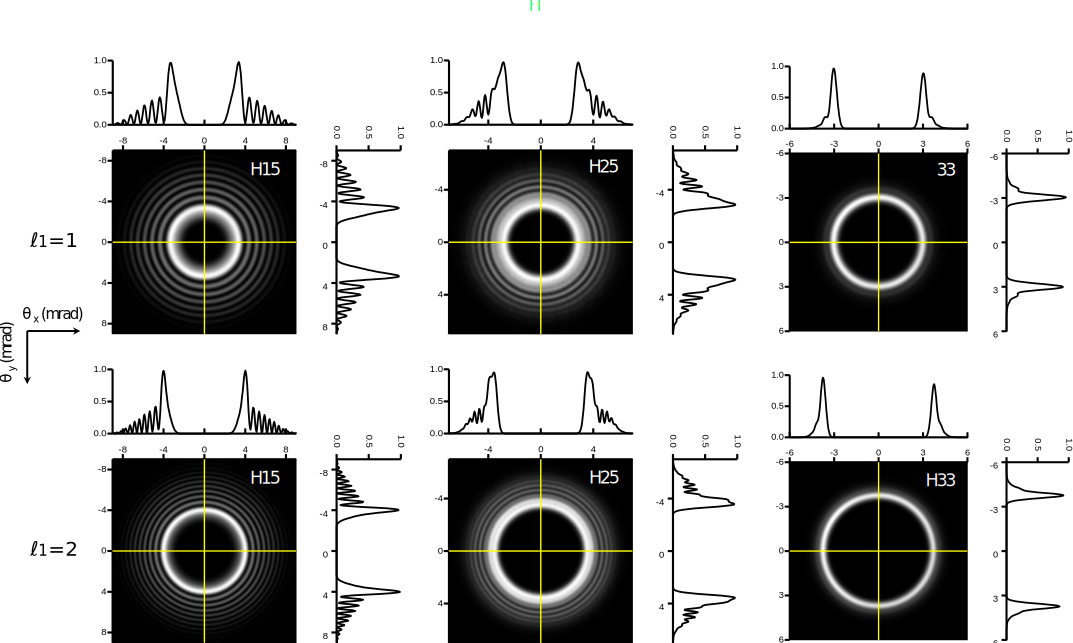
\includegraphics[width=\columnwidth]{Figures/Simul_LG_TA/FarFieldProfiles}%
\caption{Profil transverse d'intensité des harmoniques 15, 25 et 33 propagé 80 cm après le milieu de génération. Le laser infrarouge porte respectivement $\ell_1=1$ et 2 sur la ligne du haut et du bas. Des coupes des profils sont réalisées selon les lignes jaunes.}%
\label{Fig:FarFieldSimu}%
\end{figure}


Contrairement aux profils expérimentaux, ces images présentent une série d'anneaux concentriques autour d'un anneau central. Pour réaliser ce calcul SFA, qui prend en compte toutes les trajectoires quantiques de la GHOE, on a choisit de focaliser le faisceau infrarouge au milieu du gaz de génération. Dans cette condition, on sait que les trajectoires courtes et longues contribuent toutes les deux à l'émission. Nous allons voir que la différence entre simulation et expérience s'explique par des poids relatifs différents des deux trajectoires.

\section{Rôle des trajectoires quantiques dans la GHOE à partir de faisceaux de Laguerre-Gauss}
\subsection{Observation des contributions des différentes trajectoires quantiques à partir des calculs numériques}
Comme la position $z_0$ du foyer infrarouge par rapport au jet de gaz contrôle le poids relatif des trajectoires, nous faisons varier ce paramètre dans la simulation numérique. La figure \ref{Fig:H21_traj}~(a-c) présente le profil obtenu en champ lointain lorsque le laser est focalisé en amont, au milieu, et en aval du jet. Quand $z_0<0$, c'est-à-dire que le laser est focalisé avant le jet, l'accord de phase favorise fortement la trajectoire courte. Dans ce cas, le profil en champ lointain ne présente qu'un seul anneau : comme dans l'expérience on génère un mode de Laguerre-Gauss quasiment pur.

\begin{figure}[!ht]
\centering
\def\svgwidth{.7\columnwidth}
\import{Figures/Simul_LG_TA/}{trajectories.pdf_tex}
\caption{Contributions des différentes trajectoires quantiques dans la GHOE par faisceau LG. Le profil d'intensité de l'harmonique 21 est présenté pour (a) $z_0<0$, (b) $z_0=0$, (c) $z_0>0$. La convention de signe est illustrée au-dessus. Les profils (d) et (e) sont calculés avec $z_0=0$ en ne prenant en compte que la contribution respectivement de la trajectoire courte et longue.}
\label{Fig:H21_traj}
\end{figure}






\subsection{Observation expérimentale de ces contributions}
\subsection{Interprétation des résultats obtenus : le rôle de l'index radial des modes de Laguerre-Gauss}

\section{Le profil spatio-temporel des impulsions générées : les ``light springs''}
\subsection{Mesure de la phase spectrale de l'impulsion à partir de la technique RABBIT}
\subsection{Reconstruction du profil spatio-temporel de l'émission}

\section{Contrôle complet du moment orbital angulaire de l'émission dans un schéma à deux faisceaux}
\subsection{Lois de conservations dans un schéma à deux faisceaux}
\subsection{Dispositif colinéaire}
\subsection{Dispositif non colinéaire}

\section{Le reste?}
\subsection{Le FEL?}